\begin{figure}[t]
\centering
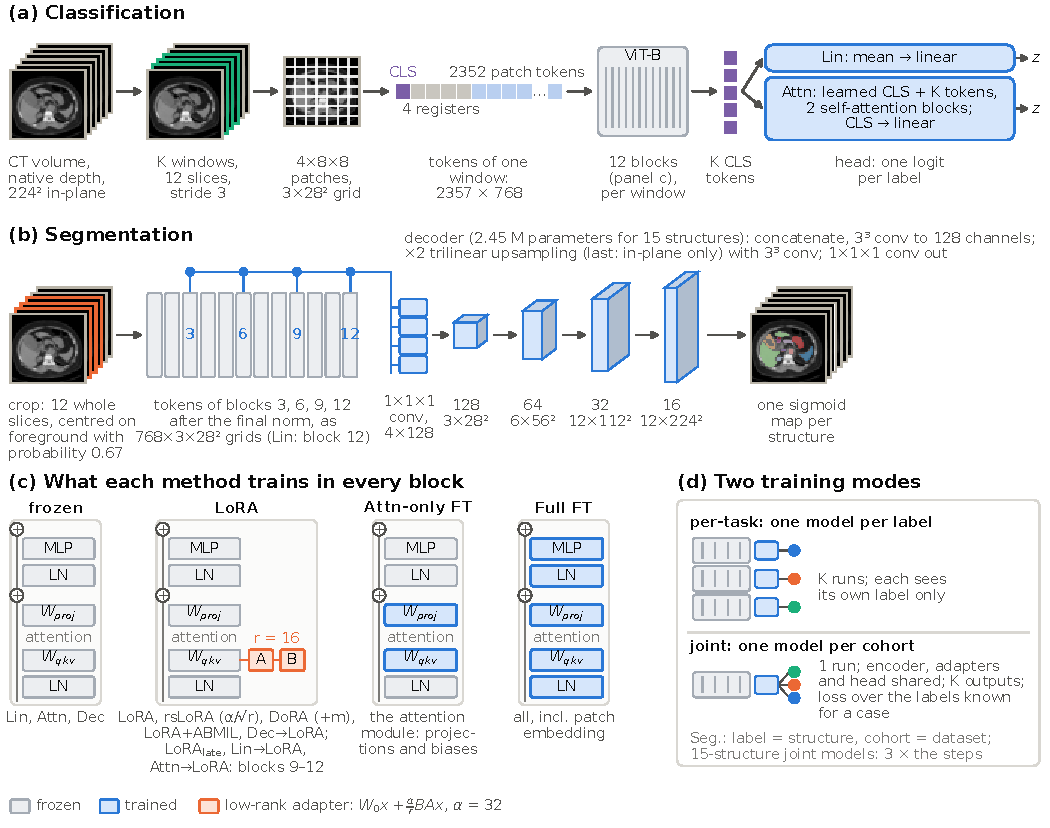
\includegraphics[width=\textwidth]{figures/fig_pipeline.pdf}
\caption{How each task is run. All panels show TAP-CT, drawn from the implementation; the other backbones are in Figures~\ref{fig:arms} and~\ref{fig:armsseg} (Appendix~\ref{app:details}). (a) Classification: 12-slice windows, $4\times8\times8$ patches; the CLS token of every window enters the head, a linear layer on their mean (Lin) or an attentive probe (Attn), with one logit per label. (b) Segmentation: the tokens of blocks 3, 6, 9 and 12 feed a multi-depth decoder (2.45\,M parameters for 15 structures) with one sigmoid map per structure (Lin uses block 12 only). (c) What each method trains in every encoder block; the head is always trained. (d) Per-task and joint training.}
\label{fig:pipeline}
\end{figure}

\paragraph{Backbones.}\label{sec:backbones} \textbf{TAP-CT-B-3D} \citep{veenboer2025tapct}, pretrained by DINOv2-style self-supervision on in-house CT, is a plain 12-block ViT-B \citep{dosovitskiy2021vit} with $4\times8\times8$ voxel patches, a CLS token and four register tokens \citep{darcet2024registers}, applied to windows of $12\times224\times224$ voxels at native slice spacing (Figure~\ref{fig:pipeline}). \textbf{SPECTRE-Large} \citep{claessens2025spectre}, pretrained by self-distillation and vision--language alignment with radiology reports, is a plain 24-block ViT-L with $16\times16\times8$ patches on $128\times128\times64$ crops; for classification, 64 crops of a $512\times512\times256$ volume at $0.5\times0.5\times1$\,mm are summarized by its pretrained 4-block feature combiner. \textbf{Pillar-0} \citep{agrawal2025pillar0}, pretrained on CT and breast MRI of one academic center, is used through its head-CT encoder, a convolutional stem followed by three stages of multi-scale window-attention blocks over the whole volume, which restricts it to the hemorrhage cohort. \textbf{VoCo-L} \citep{wu2024voco,wu2024vocolarge} is the self-supervised encoder of a SwinUNETR-v2 \citep{hatamizadeh2022swinunetr,he2023swinunetrv2}: four stages of shifted-window blocks \citep{liu2021swin} with patch merging and no class token; it encodes $96^3$ windows at 1.5\,mm, each summarized for classification by the concatenated spatial means of the stage-2 to stage-4 outputs (2688-d). Inputs follow each model's own orientation, spacing and intensity normalization (Figure~\ref{fig:arms} and Appendix~\ref{app:details}).

\paragraph{Classification methods.}\label{sec:ladder} The methods differ only in what is trained (Figures~\ref{fig:pipeline}c and~\ref{fig:arms}d). \emph{Frozen probes}: \textbf{Lin}, a linear layer on a pooled feature, and \textbf{Attn}, an attentive probe \citep{bardes2024vjepa,chen2024cae} in which a learnable CLS token joins the window, crop or scale tokens and two self-attention blocks run over the set. \emph{Low-rank adapters} on the query/key/value projections, with the attentive head: \textbf{LoRA}, rank 16 ($\alpha=32$) on every block \citep{hu2022lora}; \textbf{LoRA$_{\text{late}}$}, on the last third of the blocks (the last stage for Pillar-0 and VoCo); \textbf{LoRA+ABMIL}, with tokens first pooled by gated attention \citep{ilse2018abmil}; \textbf{DoRA} \citep{liu2024dora}; and \textbf{rsLoRA} \citep{kalajdzievski2023rslora}, whose $\alpha/\sqrt{r}$ scaling is four times the LoRA scale at $r=16$. \emph{Two-stage schedules}: \textbf{Lin$\to$LoRA} and \textbf{Attn$\to$LoRA} train the probe for half the budget and then add late-block LoRA, keeping the probe's head \citep{kumar2022lpft}. \emph{Full-rank training}: \textbf{Attn-only FT} trains every parameter of the attention modules \citep{touvron2022three} and \textbf{Full FT} every parameter of the encoder, both with the attentive head.

\paragraph{Segmentation methods.}\label{sec:segmethods} Segmentation uses TAP-CT, SPECTRE and VoCo. \textbf{Lin} is a $1\times1\times1$ convolution on the deepest token grid, upsampled trilinearly; for VoCo this grid has one token per $32^3$ voxels (48\,mm), far coarser than those of the two ViTs. \textbf{Dec} is a light multi-depth decoder in the spirit of UNETR \citep{hatamizadeh2022unetr}: the token grids of four depths are projected, concatenated, fused and upsampled to the voxel grid by $3^3$ convolutions (2.4 to 2.6\,M parameters, no skip connections from the input; Figures~\ref{fig:pipeline}b and~\ref{fig:armsseg}). LoRA, LoRA$_{\text{late}}$ and DoRA add the adapters of classification under Dec, Full FT trains the encoder with it, and Dec$\to$LoRA trains Dec for half the budget before adding all-block LoRA. Predictions are independent sigmoids per structure.

\paragraph{Per-task and joint training.} Every cohort and dataset is trained in two modes with identical data and selection (Figure~\ref{fig:pipeline}d): \emph{per-task}, one model per label or structure, and \emph{joint}, one model with shared encoder, adapters and head and one output per label or structure. A \emph{label--mode pair} is one label (or structure) on one backbone in one mode. Joint losses sum over the labels known for a case, as in per-task training, and average over structures (Equations~\ref{eq:lcls} and~\ref{eq:lseg}).
